\chapter{Sicherheit in der Softwareentwicklung}
Wird Software neu entwickelt oder werden Änderungen vorgenommen, ist es von hoher Bedeutung, die Sicherheit zu haben, dass alles wie erwartet funktioniert.
Egal wie erfahren ein Entwickler sein mag, Fehler sind unausweichlich.\\
Um mehr Sicherheit zu erlangen, werden im Folgenden Maßnahmen vorgestellt, die Funktionstüchtigkeit von Softwareprojekten gewährleisten. Insbesondere im Kontext von Refactoring spielt dies eine wichtige Rolle, da dort oft umfassende Änderungen vorgenommen werden \citep[S. 323]{fiveLines.2023}.
\section{Verschiedene Arten von Tests}
Die einfachste und verbreitetste Möglichkeit, die Korrektheit von etwas zu überprüfen, ist das Testen. Auch in der Softwareentwicklung ist dies der Fall. Allerdings ist es hier nicht so einfach, wie es sich anhört: Rund die Hälfte der Entwicklungszeit wird in das Testen investiert \citep[Introduction]{artoftesting.2011}.\\
Es gibt viele verschiedene Arten, um Software zu testen, wobei diese sich auf unterschiedlichen Ebenen bewegen. Die folgende Auflistung soll einen Überblick darüber geben. 
\begin{itemize}
  \item \textbf{Unit-Tests} (oder Modultests) sind ein Prozess, bei dem die einzelnen Unterprogramme, Unterroutinen, Klassen oder Funktionen in einem Programm getestet werden. Der Test wird also nicht auf das gesamte Programm gerichtet, sondern nur auf kleinere Bausteine \citep[S. 85]{artoftesting.2011}.
  \item \textbf{Integrations Tests} sollen das Zusammenspiel von einzelnen Modulen, aus dem vorherigen Schritt, testen. Oft ist es der Fall, dass Integrations Tests nicht separat durchgeführt werden, sondern die Stellen durch umfangreichere Unit-Tests beretis abgedeckt werden \citep[S. 117 f.]{artoftesting.2011}.
  \item \textbf{Funktionale Tests} sind ein Prozess, um Abweichungen zwischen dem Programm und der externen Spezifikation zu finden. Eine externe Spezifikation beschreibt das Verhalten des Programms aus der Sicht des Endbenutzers. Diese Tests werden normalerweise als Black-Box-Test durchgeführt, da das interne Verhalten des Codes in den vorherigen Schritten überprüft wurde. \citep[S. 119]{artoftesting.2011}
\end{itemize}
Diese Liste ist unvollständig, da nur Test-Arten gelistet sind, die den Code direkt betreffen. Es gibt zusätlich noch \textbf{System Tests}, \textbf{Akzeptantz Tests} und \textbf{Installations Tests}. Diese zielen eine höhere Ebene an und sollen die Software als ganzes Testen um festzustellen, ob die angeforderten Problemstellungen des Kunden richtig erfüllt werden und somit z.B.: Missverständnisse bei den Anforderungen ausgeschlossen werden können.
Es ist wichtig zu verstehen, dass diese Ebenen unabhänig voneinander laufen müssen. Funktionieren alle Unit-Tests ordnungsgemäß, heißt das nicht, dass die Software insgesamt funktioniert, da z.B.: Klassen falsch verwendet werden können.\\
\begin{singlespace}
\textit{„[Außerdem bleibt immer] das Risko, dass unsere Tests genau die Stelle, an der ein Fehler auftritt, nicht abdecken oder dass sie etwas anderes testen, als wir glauben.“} \citep[S. 323]{fiveLines.2023}\\
\end{singlespace}
\par
Um den Zeitaufwand des Testens auf lange Sicht geringer zu halten, gibt es wie in \citep[S. 323]{fiveLines.2023} beschrieben, die Möglichkeit das Testen zu automatisieren.\\
Um noch einen Schritt weiter zu gehen hat sich in der modernen Softwarentwicklung das Konzept der „Continous Integration“ (CI) etabliert. Dabei muss jeder Commit oder jeder Pull Request vorher definierte Aufgaben erfolgreich absolvieren. Unit-Tests, Buildvorgänge und automatisches Deployment sind dabei häufig Bestandteile.
Das kontinuierliche Durchlaufen der Tests, ermöglicht eine frühzeitige Erkennung von auftretenden Fehlern \cite{CIMeyer.2014}.
\section{Wekzeuge in der Entwicklungsumgebung}
\begin{wrapfigure}{r}{0.4\textwidth}
  \centering
  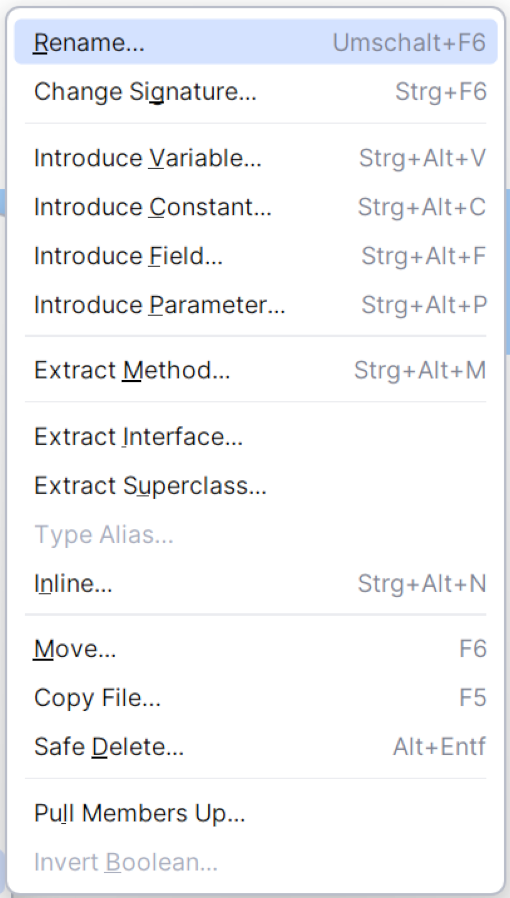
\includegraphics[width=0.35\textwidth]{Bilder/screenshotWebstorm} % Replace with your image file
  \caption{Screenshot WebStorm Refactoring-Tools \cite{webstorm.2024}}
  \label{webstormRefactor}
\end{wrapfigure}
Softwareentwicklung ist ein zeitaufwendiger Prozess, in dem es schnell zu Fehlern kommen kann. Um diese zu vermeiden, wurden verschiedenste Werkzeuge entwickelt, die die Programmierenden unterstützen sollen.
Moderne IDEs (Integrated Development Environments) haben das Ziel die Entwicklungsgeschwindigkeit zu erhöhen und Fehler zu vermeiden.
Sie kombinieren eine Vielzahl dieser hilfreichen Werkzeuge in einem einzelnen Programm. Darunter gehören unter anderem Syntax-Highlighting, Autovervollständigung, Debugging-Tools und und andere Überprüfungen, die kontinuierlich im Hintergrund laufen.
Auch Werkzeuge, die der Entwickler bewusst einsetzen kann, werden angeboten. Dazu gehören zum Beispiel Versionsverwaltung und Refactoring-Tools \citep[S. 275]{modernIDEs.2022}.\\
Die nebenstehende Abbildung \ref{webstormRefactor} zeigt das Kontextmenü für Refactoring Hilfen in der IDE WebStorm. Hier kann der Entwickler verschiedene Aktionen auswählen, die dann automatisiert durchgeführt werden.
\newpage
Ein Beispiel dafür ist die Namensänderung eines markierten Feldes. Dabei kann ein neuer Name eingegeben werden und die IDE ändert alle Stellen, an denen das Feld verwendet wird, automatisch ab.
Diese Unterstützung wird für die meisten gängigen Refactorings angeboten.\cite{webstorm.2024}
Trotzdem ist es wichtig, sich nicht vollständig auf diese Werkzeuge zu verlassen. Vorgenommene Änderungen sollten immer überprüft werden, da auch diese Tools fehlerhaft sein können \citep[S. 323 f.]{fiveLines.2023}. 

\section{Formale Verifikation der Software}
Die nächste Thematik spielt vor allem bei besonders kritischer Software eine Rolle.
Beispiele hierfür sind Systeme, von denen Menschenleben abhängen, oder bei denen erhebliche Geldsummen im Spiel sind, wie Flugzege oder der nächste Marsrover \citep[S. 324]{fiveLines.2023}.\\
Formale Verifikation beschreibt das Erheben einer Beweisführung über die Funktionstüchtigkeit von Code. Alle möglichen Ausgänge eines Programms müssen auf mathematischer Ebene bewiesen werden \cite{glinz2004formale}.
Da dieser Prozess extrem zeitaufwendig ist und Fehler in der Beweisführung unter allen Umständen vermieden werden sollten, gibt es auch hier spezielle Werkzeuge, die den Entwickler unterstützen und die Berechnungen auf Richtigkeit überprüfen.
Auch hier gilt, kommt externe Software zum Einsatz, sind Fehler dieser nicht grundsätzlich auszuschließen \citep[S. 324]{fiveLines.2023}.

\section{Eine Fehlertoleranz einbauen}
Der letzte Ansatz, der untersucht werden soll, bezieht sich auf eine gewisse Fehlertoleranz der Software.
Es gibt mehrere Möglichkeiten, diese in Code einzubauen. 
Eine davon ist das Verwenden von Feature-Schaltern. Diese können im Fehlerfall komplette Funktionaltäten deaktivieren, um die Software weiterhin lauffähig zu halten.
Alternativ kann auch ein Mechanismus eingebaut werden, der bei einem Fehler auf eine ältere stabile Version der Software zurückgreift \citep[S. 324]{fiveLines.2023}. \\
Leider gewährleistet auch dieses Vorgehen keine 100-prozentige Sicherheit, da Fehler falsch erkannt werden können.\\
\begin{singlespace}
\textit{„Ein Beispiel hierfür wäre eine Funktion, die im Fehlerfall -1 zurückgibt, anstatt einen Fehler zu werfen. Das System erwartet vielleicht eine ganze Zahl, und -1 passt zu dieser Erwartung.“} \citep[S. 324]{fiveLines.2023}.\\
\end{singlespace}
\par
Zusammenfassend lässt sich sagen, dass es viele verschiedene Möglichkeiten gibt, die Sicherheit von Software zu gewährleisten. Jedoch ist keine dieser Methoden fehlerfrei. Es ist wichtig, mehrere dieser Ansätze zu kombinieren, um die Wahrscheinlichkeit von Fehlern zu minimieren.
Diese Beobachtung speißt die Aussage, dass Software nie fertig ist, da in ihrer Lebenszeit immer wieder neue Fehler entdeckt werden, die behoben werden müssen.